% !TeX root = RJwrapper.tex
\title{Calendar-based graphics for visualizing people's daily schedules}
\author{by Earo Wang, Dianne Cook, Rob J Hyndman}

\maketitle

\abstract{%
Calendars are broadly used in society to display temporal information,
and events. This paper describes a new R package with functionality to
organize and display temporal data, collected on sub-daily resolution,
into a calendar layout. The function \code{frame\_calendar} uses linear
algebra on the date variable to restructure data into a format lending
itself to calendar layouts. The user can apply the grammar of graphics
to create plots inside each calendar cell, and thus the displays
synchronize neatly with \pkg{ggplot2} graphics. The motivating
application is studying pedestrian behavior in Melbourne, Australia,
based on counts which are captured at hourly intervals by sensors
scattered around the city. Faceting by the usual features such as day
and month, was insufficient to examine the behavior. Making displays on
a monthly calendar format helps to understand pedestrian patterns
relative to events such as work days, weekends, holidays, and special
events. The layout algorithm has several format options and variations.
It is implemented in the R package \pkg{sugrrants}.
}


\hypertarget{introduction}{%
\section{Introduction}\label{introduction}}

We develop a method for organizing and visualizing temporal data,
collected at sub-daily intervals, into a calendar layout. The calendar
format is created using linear algebra, giving a restructuring of the
data, that can then be piped into grammar of graphics definitions of
plots, as used in \CRANpkg{ggplot2} (Wickham et al. 2018). The data
restructuring approach is consistent with the tidy data principles
available in the \CRANpkg{tidyverse} (Wickham 2017) suite. The methods
are implemented in a new package called \CRANpkg{sugrrants} (Wang, Cook,
and Hyndman 2018) .

The purpose of the calendar-based visualization is to provide insights
into people's daily schedules relative to events such as work days,
weekends, holidays, and special events. This work was originally
motivated by studying foot traffic in the city of Melbourne, Australia
(City of Melbourne 2017). There have been 43 sensors installed that
count pedestrians every hour across the downtown area (Figure
\ref{fig:ped-map}). The dataset can shed light on people's daily
rhythms, and assist the city administration and local businesses with
event planning and operational management. A routine examination of the
data would involve constructing conventional time series plots to catch
a glimpse of temporal patterns. The faceted plots in Figure
\ref{fig:time-series-plot}, give an overall picture of the foot traffic
at 3 different sensors over 2016. Further faceting by day of the week
(Figure \ref{fig:facet-time}) provides a better glimpse of the daily and
sub-daily pedestrian patterns. The sensor data, like many temporal
datasets on human behaviors, lends itself to a number of exploratory
data visualization challenges:

\begin{enumerate}
\def\labelenumi{\arabic{enumi}.}
\tightlist
\item
  Variations exist on multiple time scales including time of day, day of
  week, and day of year (such as public holiday and recurring events).
\item
  Since the data are often collected at sub-daily frequencies, they
  typically involve a large number of observations.
\item
  Measurements of a single type are made at multiple locations at a
  given time point, which creates the need for comparing and contrasting
  between locations.
\end{enumerate}

The conventional ways to display time series and constructing faceted
displays are insufficient to address these challenges.

\begin{Schunk}
\begin{figure}

{\centering 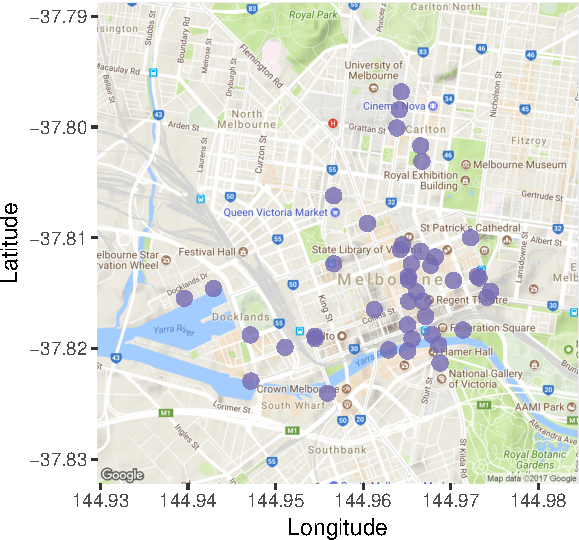
\includegraphics[width=0.7\linewidth]{figure/ped-map-1} 

}

\caption[Map of the Melbourne city area with dots indicating sensor locations]{Map of the Melbourne city area with dots indicating sensor locations. 3 sensors have been highlighted to give a closer look at in the paper.}\label{fig:ped-map}
\end{figure}
\end{Schunk}

\begin{Schunk}
\begin{figure}

{\centering 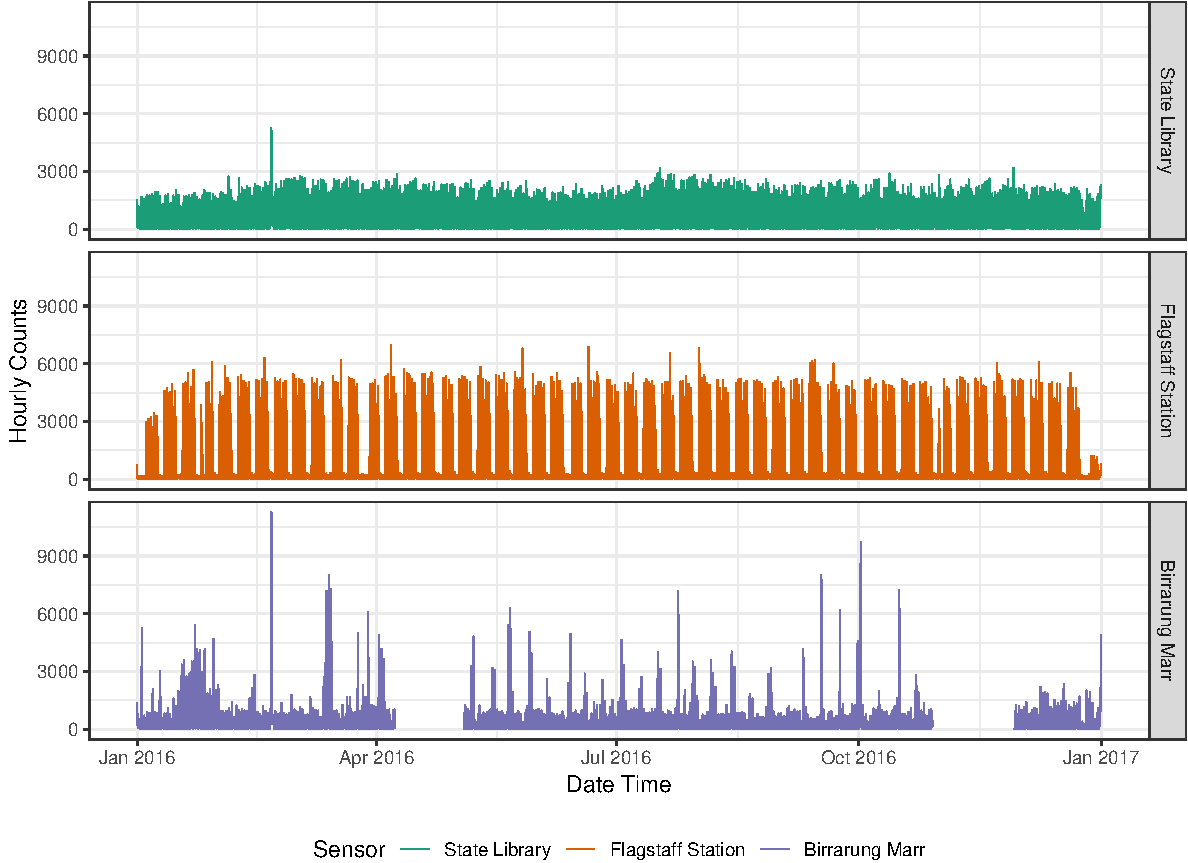
\includegraphics[width=\textwidth]{figure/time-series-plot-1} 

}

\caption[Time series plots showing the number of pedestrians in 2016 measured at 3 different sensors in the city of Melbourne]{Time series plots showing the number of pedestrians in 2016 measured at 3 different sensors in the city of Melbourne. Colored by the sensors, small multiples of lines show that the foot traffic varies from one sensor to another in terms of both time and number. The weekly patterns look distinctive across these 3 sensors. There is an eye-catching spike which occurred at the State Library, caused by the annual White Night event on 20th of February.}\label{fig:time-series-plot}
\end{figure}
\end{Schunk}

\begin{Schunk}
\begin{figure}

{\centering 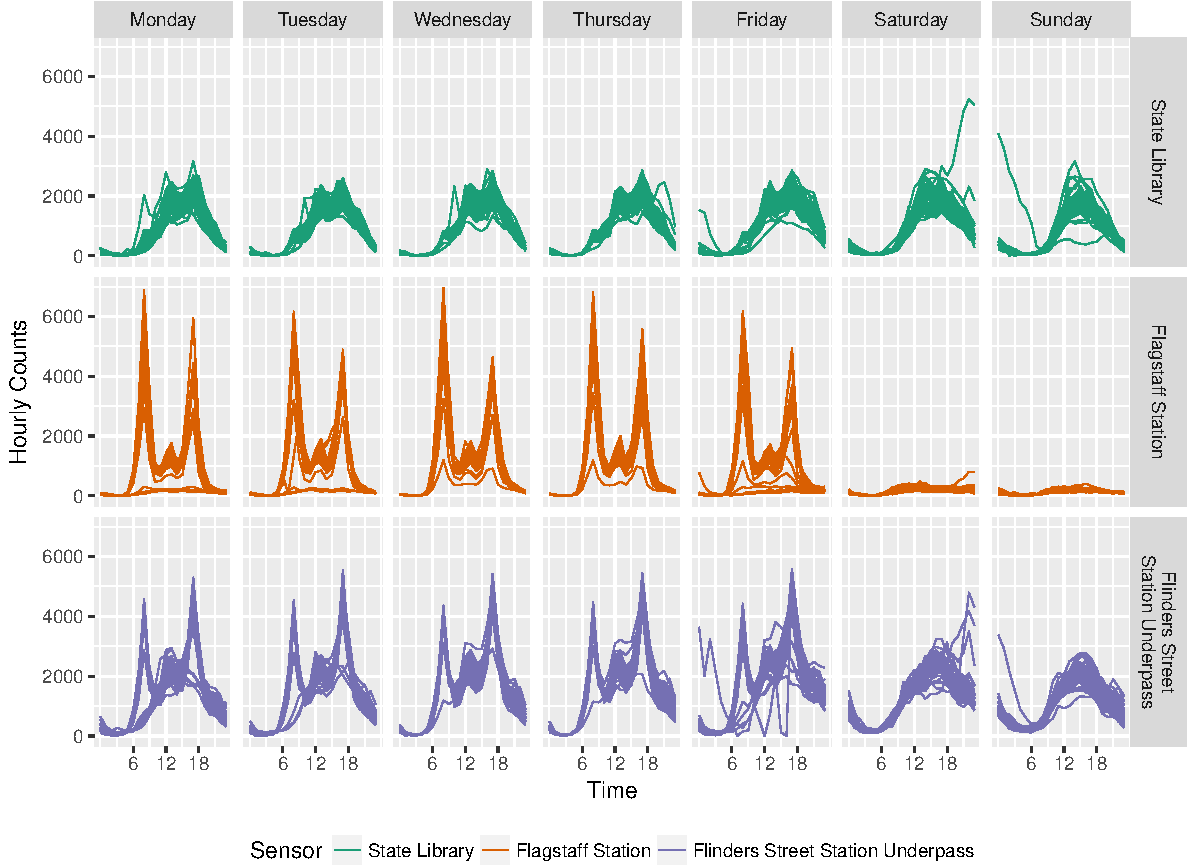
\includegraphics[width=\textwidth]{figure/facet-time-1} 

}

\caption[Hourly pedestrian counts for 2016 faceted by sensors and days of the week using lines]{Hourly pedestrian counts for 2016 faceted by sensors and days of the week using lines. It features at least two types of seasons---time of day and day of week---across all the sensors. The White Night effect on increasing pedestrian counts can be seen on Saturday in February at the State Library.}\label{fig:facet-time}
\end{figure}
\end{Schunk}

The work is inspired by Wickham et al. (2012), which uses linear algebra
to display spatio-temporal data as glyphs on maps. It is also related to
recent work by Hafen (2018) which provides methods in the
\CRANpkg{geofacet} package to arrange data plots into a grid, while
preserving the geographical position. Both of these show data in a
spatial context.

In contrast, calendar-based graphics unpack the temporal variable, at
different resolutions, to digest multiple seasonalities, and special
events. There is some existing work in this area. For example, Van Wijk
and Van Selow (1999) developed a calendar view of the heatmap to
represent the number of employees in the work place over a year, where
colors indicate different clusters derived from the days. It contrasts
week days and weekends, highlights public holidays, and presents other
known seasonal variation such as school vacations, all of which have
influence over the turn-outs in the office. The calendar-based heatmap
was implemented in two R packages: \pkg{ggTimeSeries} (Kothari and Ather
2016) and \pkg{ggcal} (Jacobs 2017). However, these techniques are
limited to color-encoding graphics and are unable to use time scales
smaller than a day. Time of day, which serves as one of the most
important aspects in explaining substantial variations arising from the
pedestrian sensor data, will be neglected through daily aggregation.
Additionally, if simply using colored blocks rather than curves, it may
become perceptually difficult to estimate the shape positions and
changes, although using curves comes with the cost of more display
capacity (Cleveland and McGill 1984; Lam, Munzner, and Kincaid 2007).

We propose a new algorithm to go beyond the calendar-based heatmap. The
approach is developed with three conditions in mind: (1) to display
time-of-day variation in addition to longer temporal components such as
day-of-week and day-of-year; (2) to incorporate line graphs and other
types of glyphs into the graphical toolkit for the calendar layout; (3)
to enable overlaying plots consisting of multiple time series. The
proposed algorithm has been implemented in the \code{frame\_calendar}
function in the \pkg{sugrrants} package using R.

The remainder of the paper is organized as follows. Section
\ref{sec:algorithm} demonstrates the construction of the calendar layout
in depth. Section \ref{sec:opt} lists and describes the options that
come with the \code{frame\_calendar} function. Section
\ref{sec:examples} presents some variations of its usage. Section
\ref{sec:discussion} discusses the advantages and disadvantages of the
method.

\hypertarget{construction}{%
\section{Construction}\label{construction}}

\label{sec:algorithm}

Figure \ref{fig:flinders-2016} shows the line glyphs framed in the
monthly calendar over the year 2016. This is achieved by the
\code{frame\_calendar} function, which computes the coordinates on the
calendar for the input data variables. These can then be plotted using
the usual \pkg{ggplot2} package (Wickham et al. 2018) functions. All of
the grammar of graphics (Wilkinson 2005; Wickham 2009) can be applied.

\begin{Schunk}
\begin{figure}

{\centering 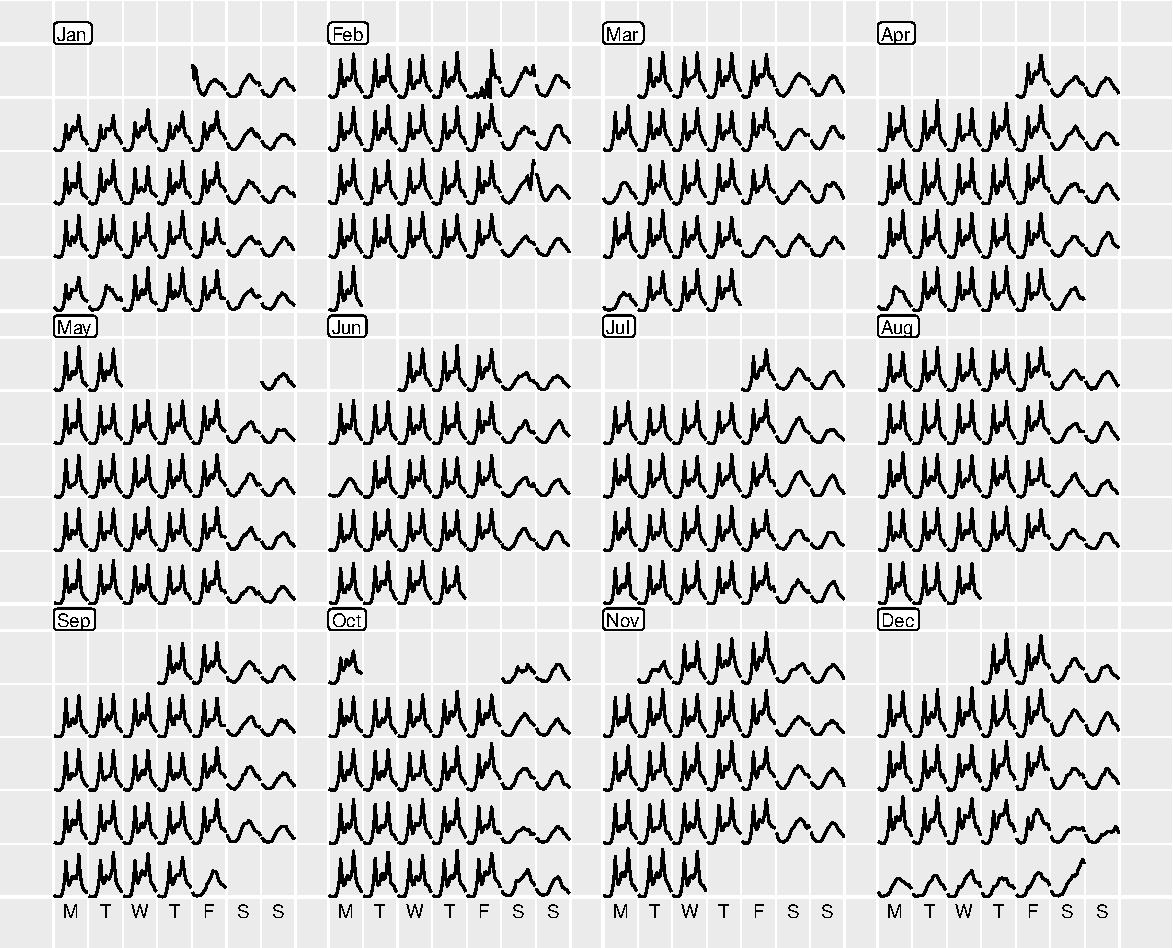
\includegraphics[width=\textwidth]{figure/flinders-2016-1} 

}

\caption[The calendar-based display of hourly foot traffic at Flinders Street Station using line glyphs]{The calendar-based display of hourly foot traffic at Flinders Street Station using line glyphs. The arrangement of the data into a 3 by 4 monthly grid represents all the traffic in 2016. The disparities between week day and weekend along with public holiday are immediately apparent.}\label{fig:flinders-2016}
\end{figure}
\end{Schunk}

The algorithm for constructing a calendar plot uses linear algebra,
similar to that used in the glyph map displays for spatio-temporal data
(Wickham et al. 2012). To make a year long calendar requires cells for
days, embedded in blocks corresponding to months, organized into a grid
layout for a year. Each month can be captured with 35 (5 \(\times\) 7)
cells, where the top left is Monday of week 1, and the bottom right is
Sunday of week 5 by default. These cells provide a micro canvas on which
to plot the data. The first day of the month could be any of
Monday--Sunday, which is determined by the year of the calendar. Months
are of different lengths, ranging from 28 to 31 days, and each month
could extend over six weeks but the convention in these months is to
wrap the last few days up to the top row of the block. The notation for
creating these cells is as follows:

\begin{itemize}
\tightlist
\item
  \(k = 1, \dots , 7\) is the day of the week that is the first day of
  the month.
\item
  \(d = 28, 29, 30\) or \(31\) representing the number of days in any
  month.
\item
  \((i, j)\) is the grid position where \(1 \le i \le 5\) is week within
  the month, \(1 \le j \le 7\), is day of the week.
\item
  \(g = k, \dots,(k+d)\) indexes the day in the month, inside the 35
  possible cells.
\end{itemize}

The grid position for any day in the month is given by

\begin{equation}
  \begin{aligned}
  i &= \lceil (g \text{ mod } 35) / 7\rceil, \\
  j &= g \text{ mod } 7. \label{eq:grid}
  \end{aligned}
\end{equation}

Figure \ref{fig:month-diagram} illustrates this \((i,j)\) layout for a
month where \(k=5\).

\begin{Schunk}
\begin{figure}

{\centering 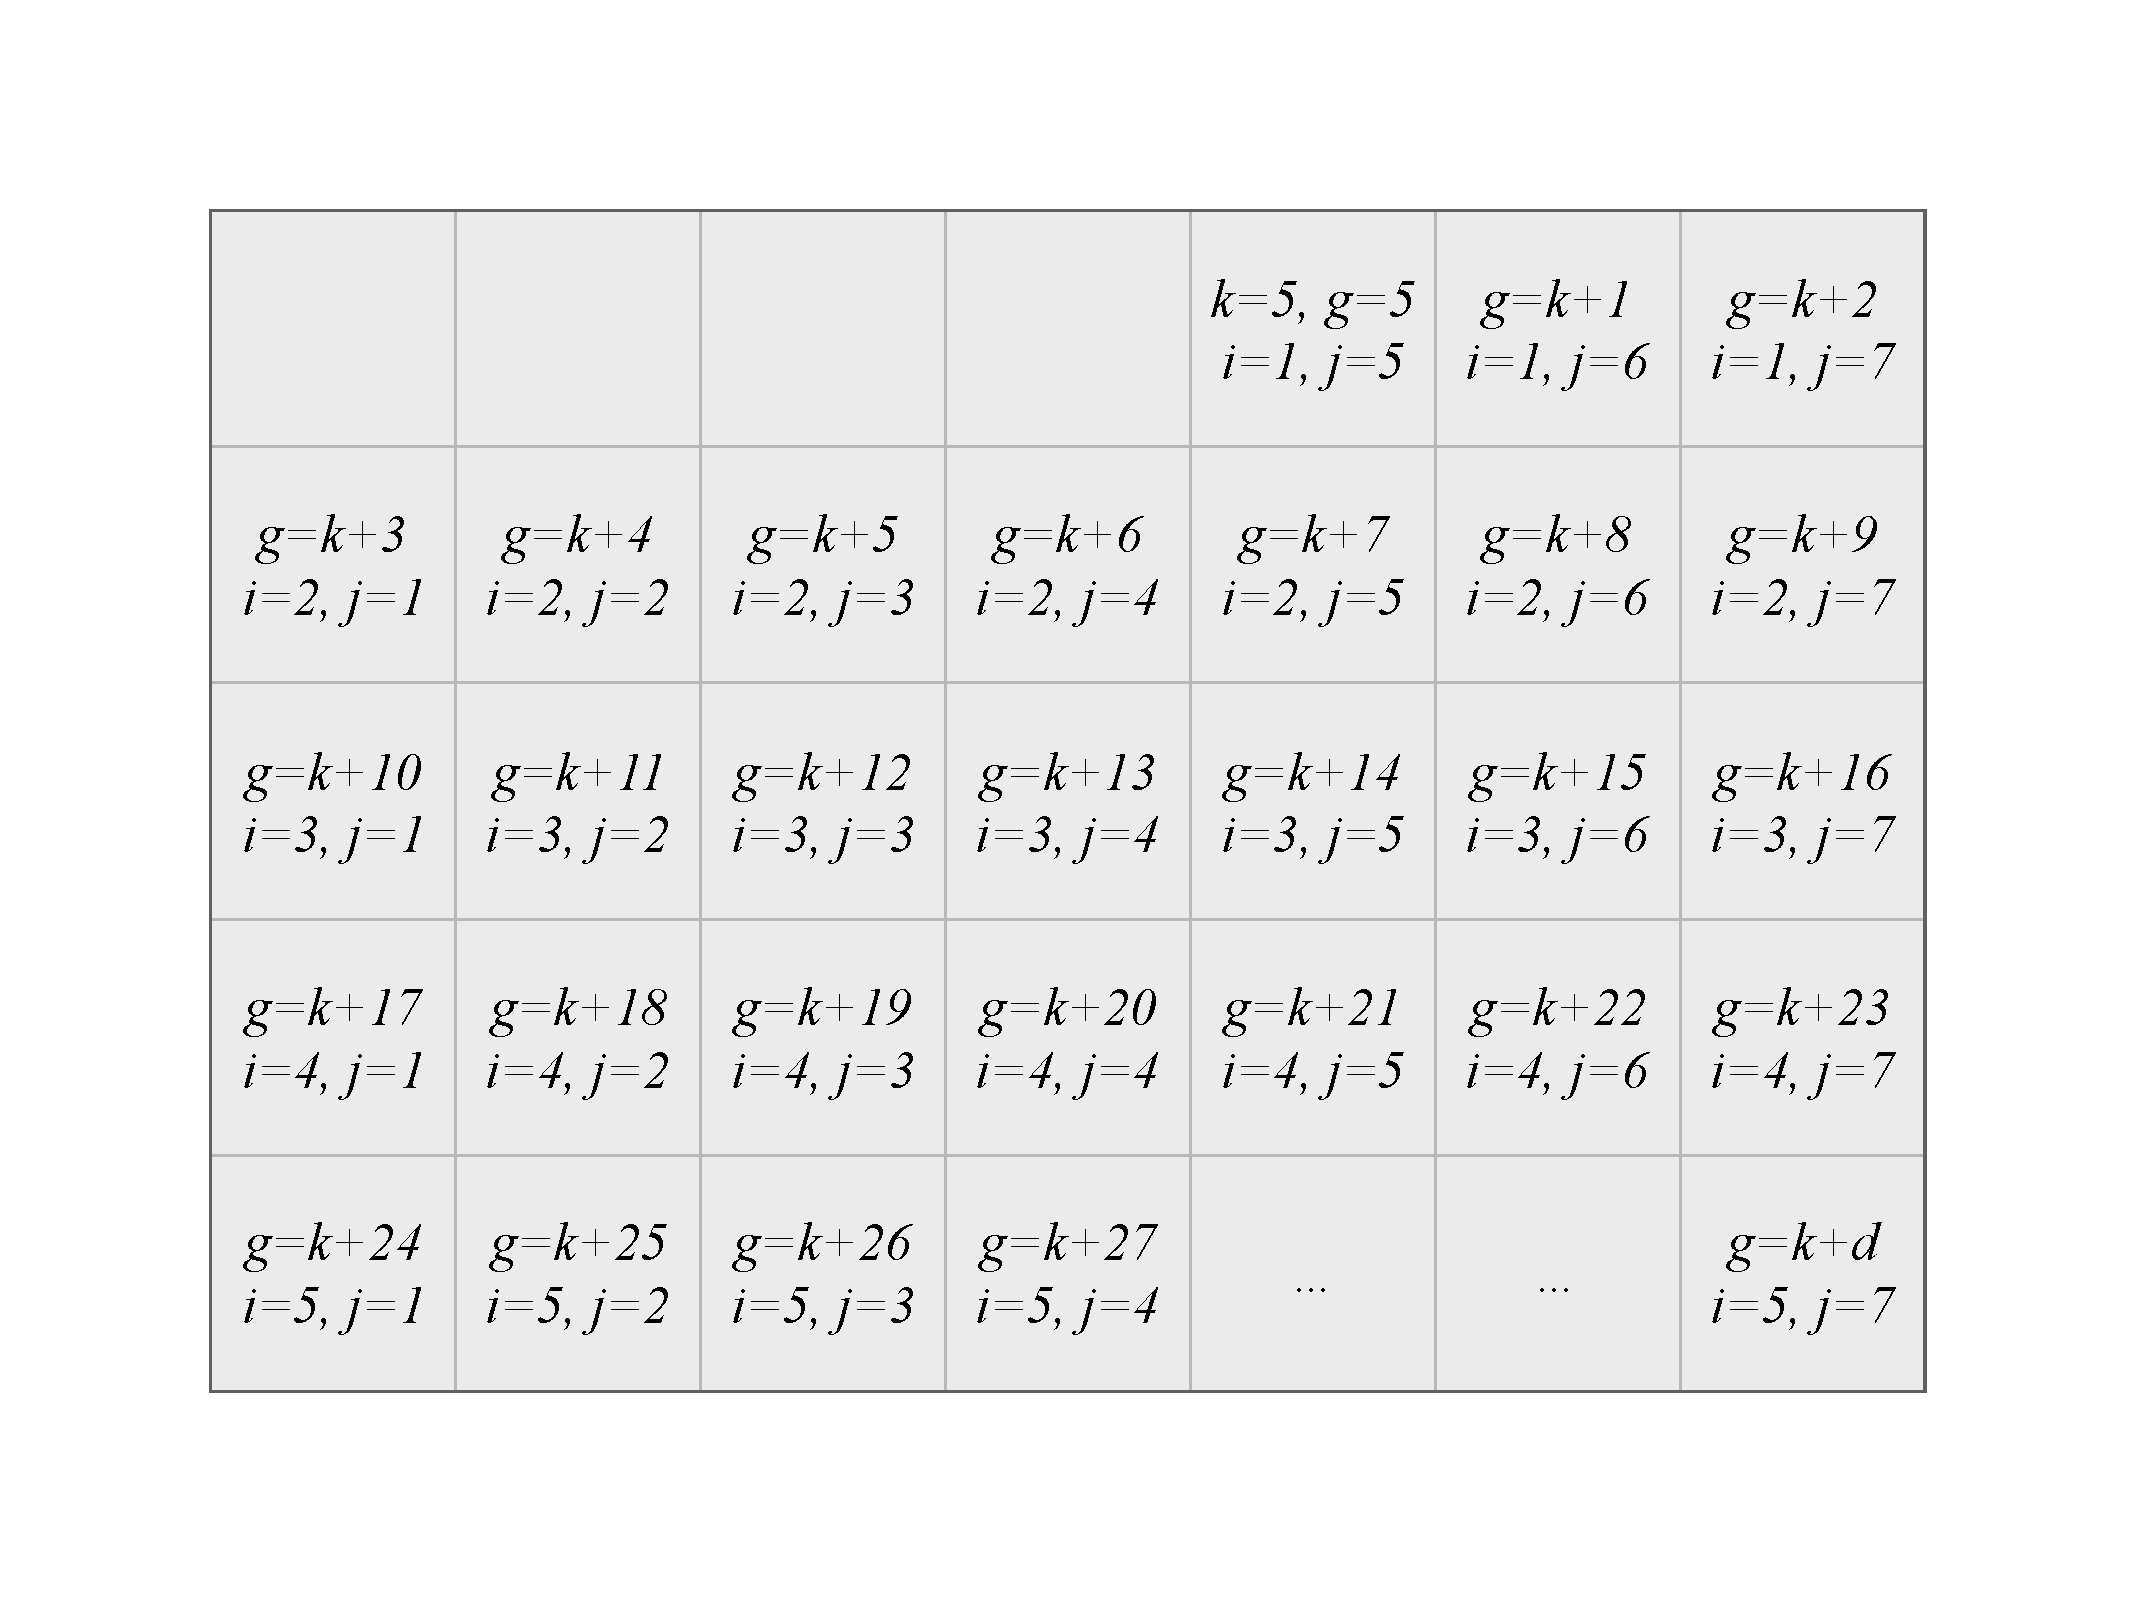
\includegraphics[width=360pt,height=250pt]{img/month} 

}

\caption[Illustration of the indexing layout for cells in a month, where $k$ is day of the week, $g$ is day of the month, $(i, j)$ indicates grid position]{Illustration of the indexing layout for cells in a month, where $k$ is day of the week, $g$ is day of the month, $(i, j)$ indicates grid position.}\label{fig:month-diagram}
\end{figure}
\end{Schunk}

To create the layout for a full year, \((m, n)\) denotes the position of
the month arranged in the plot, where \(1 \le m \le M\) and
\(1 \le n \le N\). Between each month requires some small amount of
white space, denoted by \(b\). Figure \ref{fig:year-diagram} illustrates
this layout where \(M = 3\) and \(N = 4\).

\begin{Schunk}
\begin{figure}

{\centering 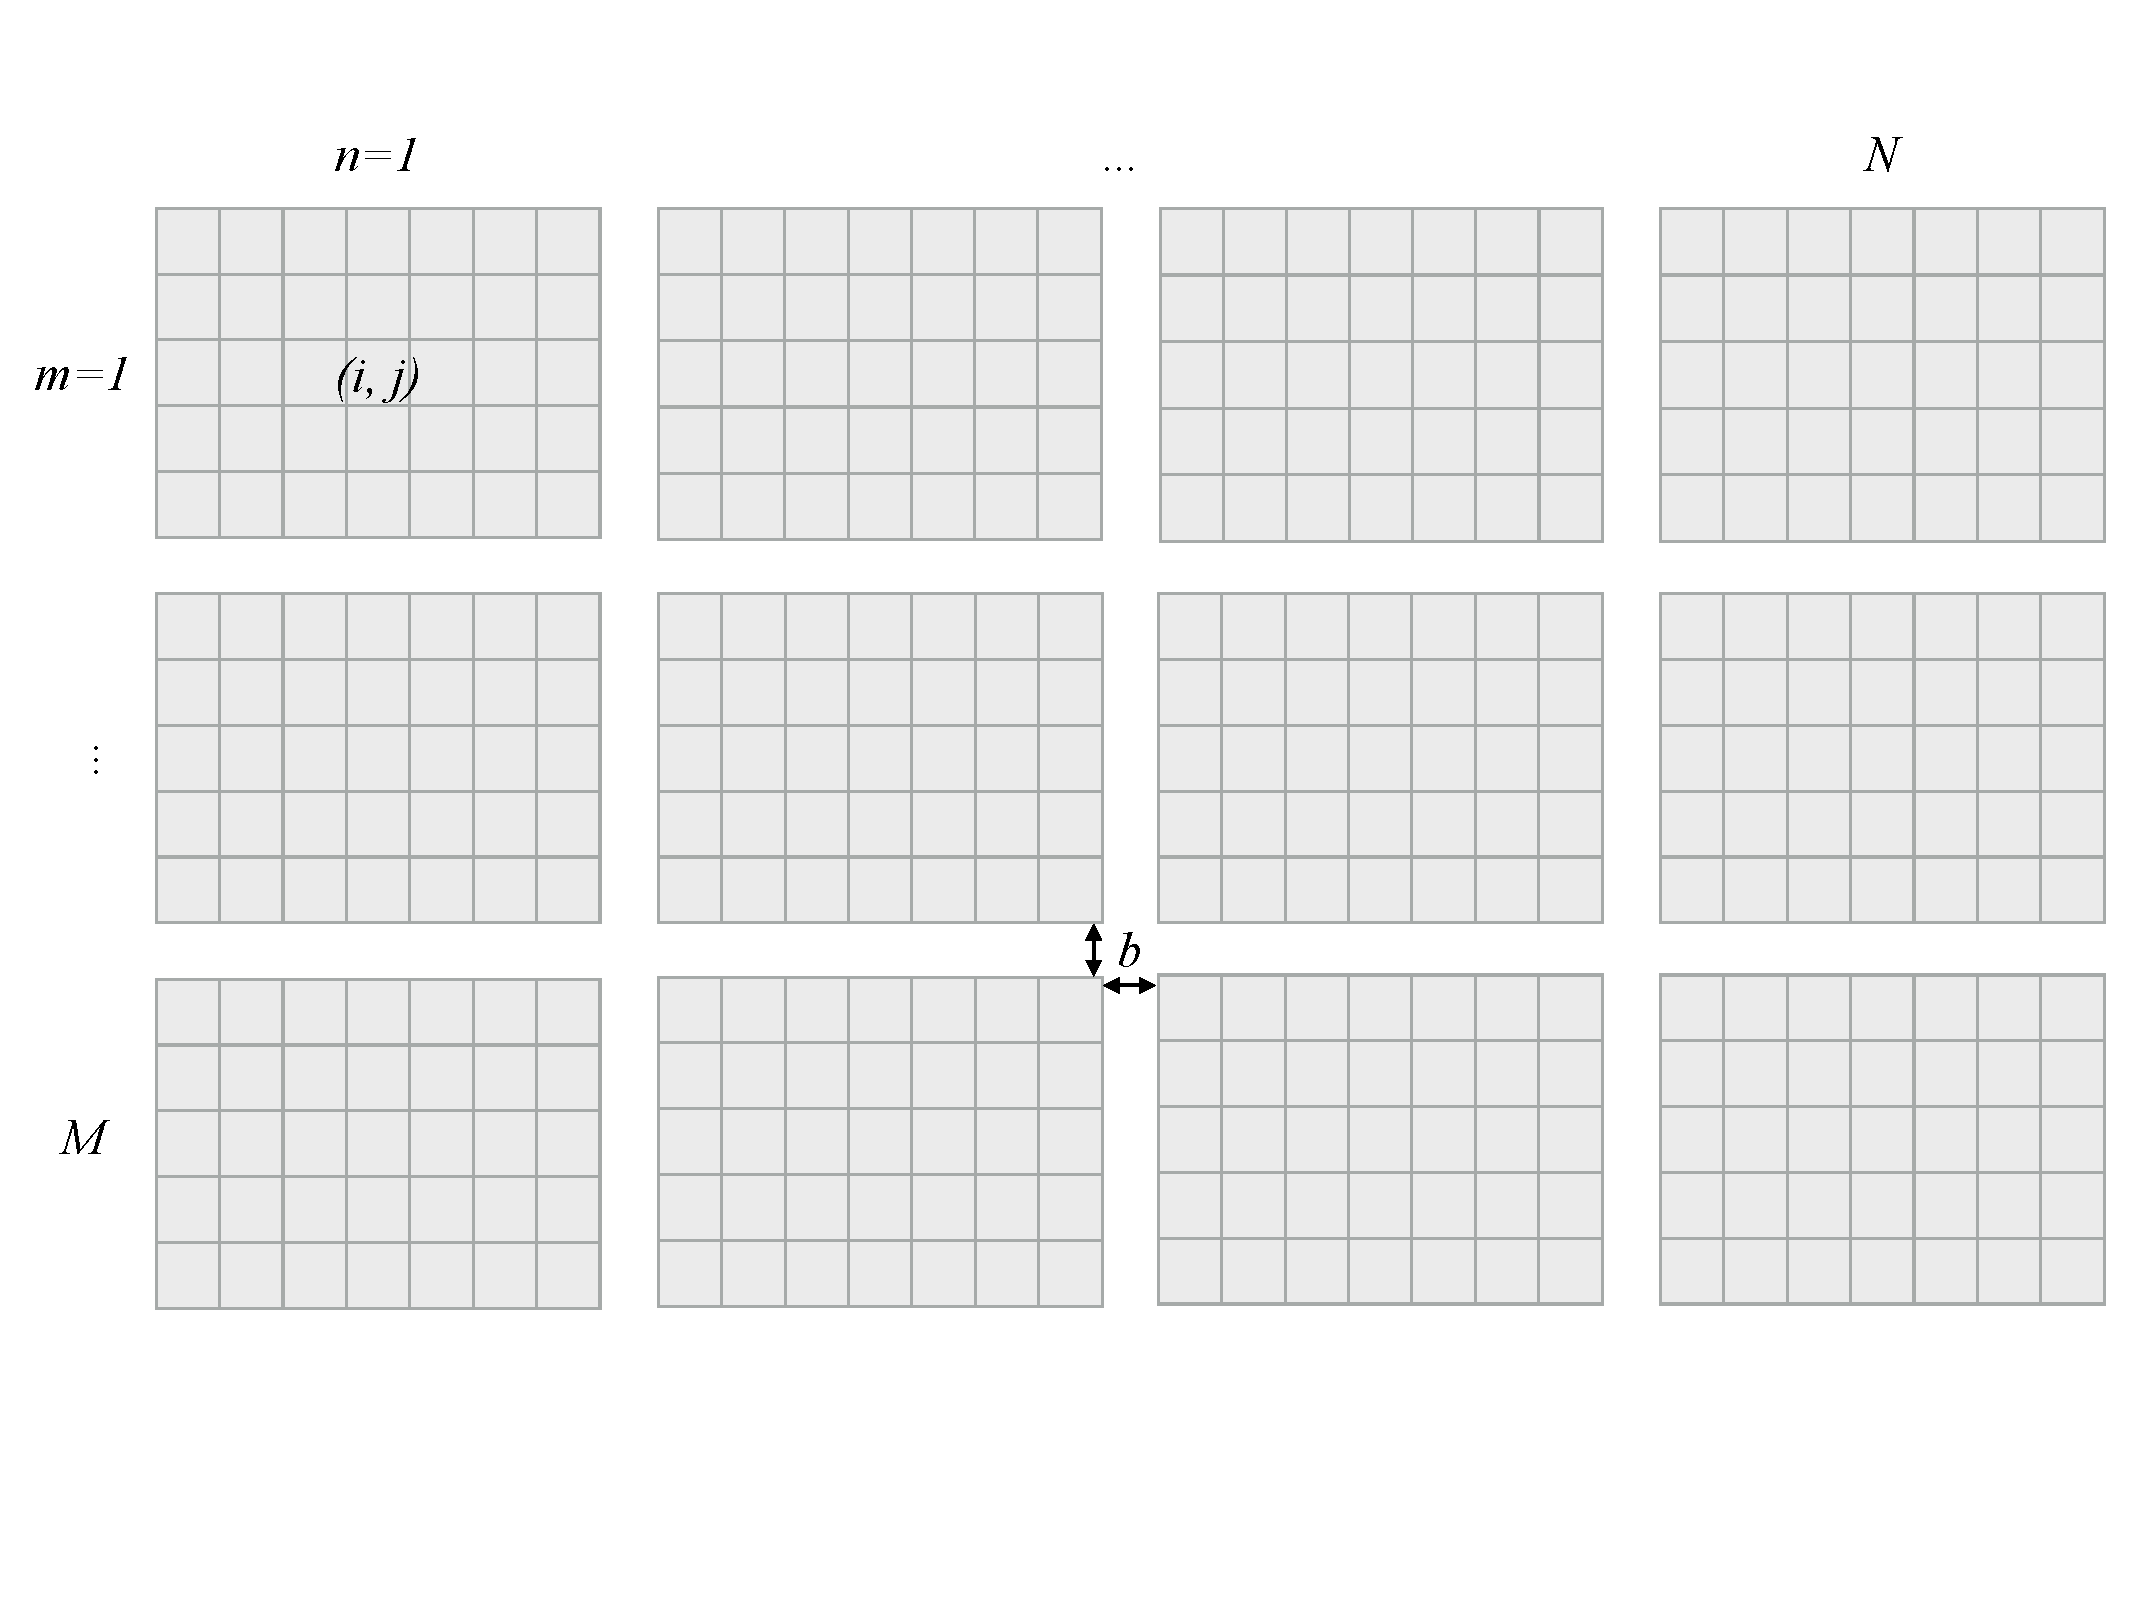
\includegraphics[width=360pt,height=250pt]{img/year-diagram} 

}

\caption[Illustration of the indexing layout for months of one year, where $M$ and $N$ indicate number of rows and columns, $b$ is a space parameter separating cells]{Illustration of the indexing layout for months of one year, where $M$ and $N$ indicate number of rows and columns, $b$ is a space parameter separating cells.}\label{fig:year-diagram}
\end{figure}
\end{Schunk}

Each cell forms a canvas on which to draw the data. Initialize the
canvas to have limits \([0, 1]\) both horizontally and vertically. For
the pedestrian sensor data, within each cell, hour is plotted
horizontally and count is plotted vertically. Each variable is scaled to
have values in \([0,1]\), using the minimum and maximum of all the data
values to be displayed, assuming fixed scales. Let \(h\) be the scaled
hour, and \(c\) the scaled count.

Then the final points for making the calendar line plots of the
pedestrian sensor data is given by:

\begin{equation}
  \begin{aligned}
  x &= j + (n - 1) \times 7 + (n - 1) \times b + h, \\
  y &= i - (m - 1) \times 5 - (m - 1) \times b + c. \label{eq:final}
  \end{aligned}
\end{equation}

Note that for the vertical direction, the top left is the starting point
of the grid (in Figure \ref{fig:month-diagram}) which is why subtraction
is performed. Within each cell, the starting position is the bottom
left.

In order to make calendar-based graphics more accessible and
informative, reference lines dividing each cell and block as well as
labels indicating week day and month are also computed before plot
construction.

Regarding the monthly calendar, the major reference lines separate every
month panel and the minor ones separate every cell, represented by the
thick and thin lines in Figure \ref{fig:flinders-2016}, respectively.
The major reference lines are placed surrounding every month block: for
each \(m\), the vertical lines are determined by \(\min{(x)}\) and
\(\max{(x)}\); for each \(n\), the horizontal lines are given by
\(\min{(y)}\) and \(\max{(y)}\). The minor reference lines are only
placed on the left side of every cell: for each \(i\), the vertical
division is \(\min{(x)}\); for each \(j\), the horizontal is
\(\min{(y)}\).

The month labels located on the top left using
\((\min{(x)}, \max{(y)})\) for every \((m, n)\). The week day texts are
uniformly positioned on the bottom of the whole canvas, that is
\(\min{(y)}\), with the central position of a cell \(x / 2\) for each
\(j\).

\hypertarget{options}{%
\section{Options}\label{options}}

\label{sec:opt}

The algorithm has several optional parameters that modify the layout,
direction of display, scales, plot size and switching to polar
coordinates. These are accessible to the user by the inputs to the
function \code{frame\_calendar}:

\begin{verbatim}
frame_calendar(
  data, x, y, date, calendar = "monthly", dir = "h", 
  sunday = FALSE, nrow = NULL, ncol = NULL, polar = FALSE, 
  scale = "fixed", width = 0.95, height = 0.95, margin = NULL
)
\end{verbatim}

It is assumed that the \texttt{data} is in tidy format (Wickham 2014),
and \code{x}, \code{y} are the variables that will be mapped to the
horizontal and vertical axes in each cell. For example, the \code{x} is
the time of the day, and \code{y} is the count (Figure
\ref{fig:flinders-2016}). The \code{date} argument specifies the date
variable used to construct the calendar layout.

The algorithm handles displaying a single month or several years. The
arguments \code{nrow} and \code{ncol} specify the layout of multiple
months. For some time frames, some arrangements may be more beneficial
than others. For example, to display data for three years, setting
\code{nrow = 3} and \code{ncol = 12} would show each year on a single
row.

\hypertarget{layouts}{%
\subsection{Layouts}\label{layouts}}

The monthly calendar is the default, but two other formats, weekly and
daily, are available with the \code{calendar} argument. The daily
calendar arranges days along a row, one row per month. The weekly
calendar stacks weeks of the year vertically, one row for each week, and
one column for each day. The reader can scan down all the Mondays of the
year, for example. The daily layout puts more emphasis on day of the
month. The weekly calendar is appropriate if most of the variation can
be characterized by days of the week. On the other hand, the daily
calendar should be used when there is a yearly effect but not a weekly
effect in the data (for example weather data). When both effects are
present, the monthly calendar would be a better choice. Temporal
patterns motivate which variant should be employed.

\hypertarget{polar-transformation}{%
\subsection{Polar transformation}\label{polar-transformation}}

When \code{polar = TRUE}, a polar transformation is carried out on the
data. The computation is similar to the one described in Wickham et al.
(2012). Figure \ref{fig:flinders-polar} shows star plots embedded in the
monthly calendar layout, which is equivalent to Figure
\ref{fig:flinders-2016} placed in polar coordinates.

\begin{Schunk}
\begin{figure}

{\centering 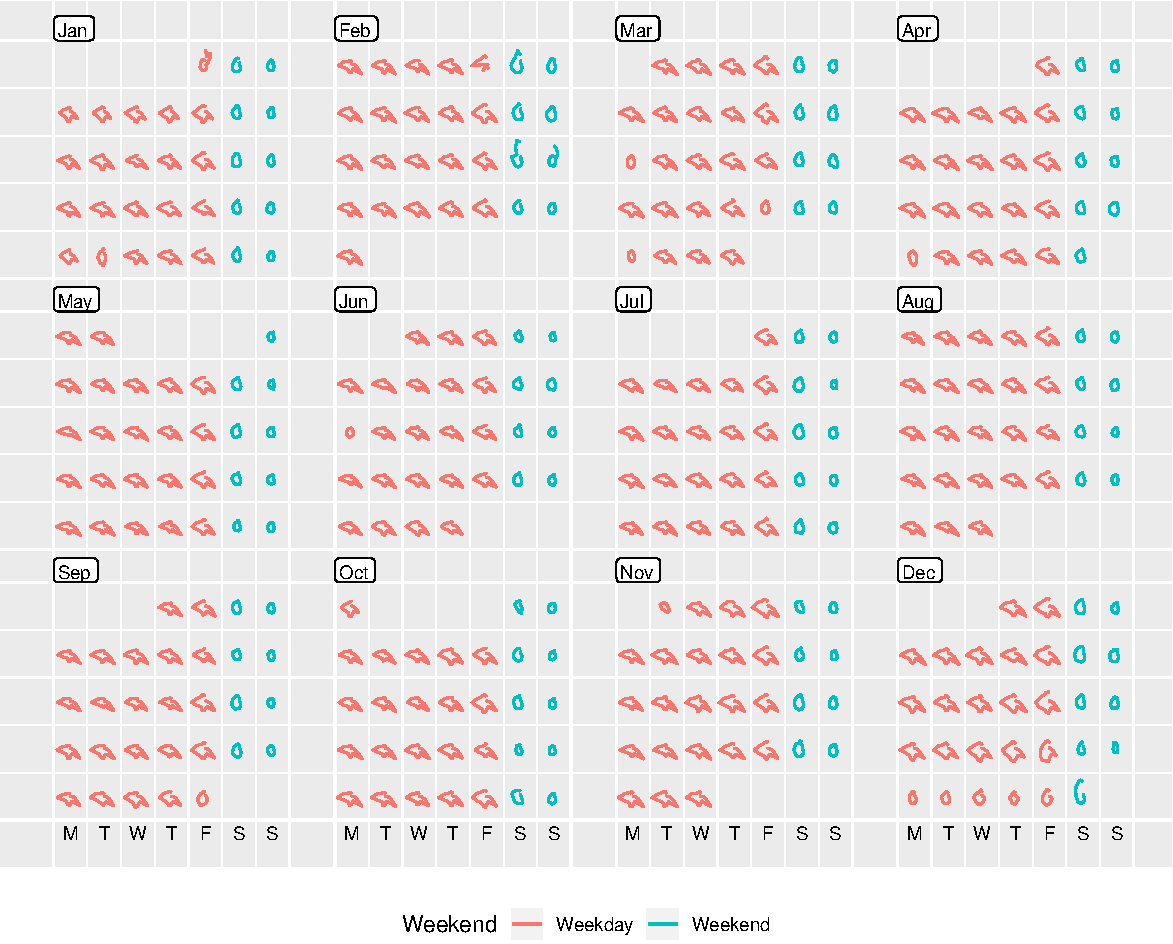
\includegraphics[width=\textwidth]{figure/flinders-polar-1} 

}

\caption{Figure \ref{fig:flinders-2016} in circular layout, which is referred to as star plots. The daily periodicity on work days are clearly visible.}\label{fig:flinders-polar}
\end{figure}
\end{Schunk}

\hypertarget{scales}{%
\subsection{Scales}\label{scales}}

By default, global scaling is done for values in each plot, with the
global minimum and maximum used to fit values into each cell. If the
emphasis is comparing trend rather than magnitude, it is useful to scale
locally. For temporal data this would harness the temporal components.
The choices include: free scale within each cell (\code{free}), cells
derived from the same day of the week (\code{free\_wday}), or cells from
the same day of the month (\code{free\_mday}). The scaling allows for
the comparisons of absolute or relative values, and the emphasis of
different temporal variations.

With local scaling, the overall variation gives way to the individual
shape. Figure \ref{fig:flinders-free} shows the same data as Figure
\ref{fig:flinders-2016} scaled locally using \code{scale = "free"}. The
daily trends are magnified.

The \code{free\_wday} scales each week day together. It can be useful to
comparing trends across week days, allowing relative patterns for
weekends versus week days to be examined. Similarly, the
\code{free\_mday} uses free scaling for any day within a given month.

\begin{Schunk}
\begin{figure}

{\centering 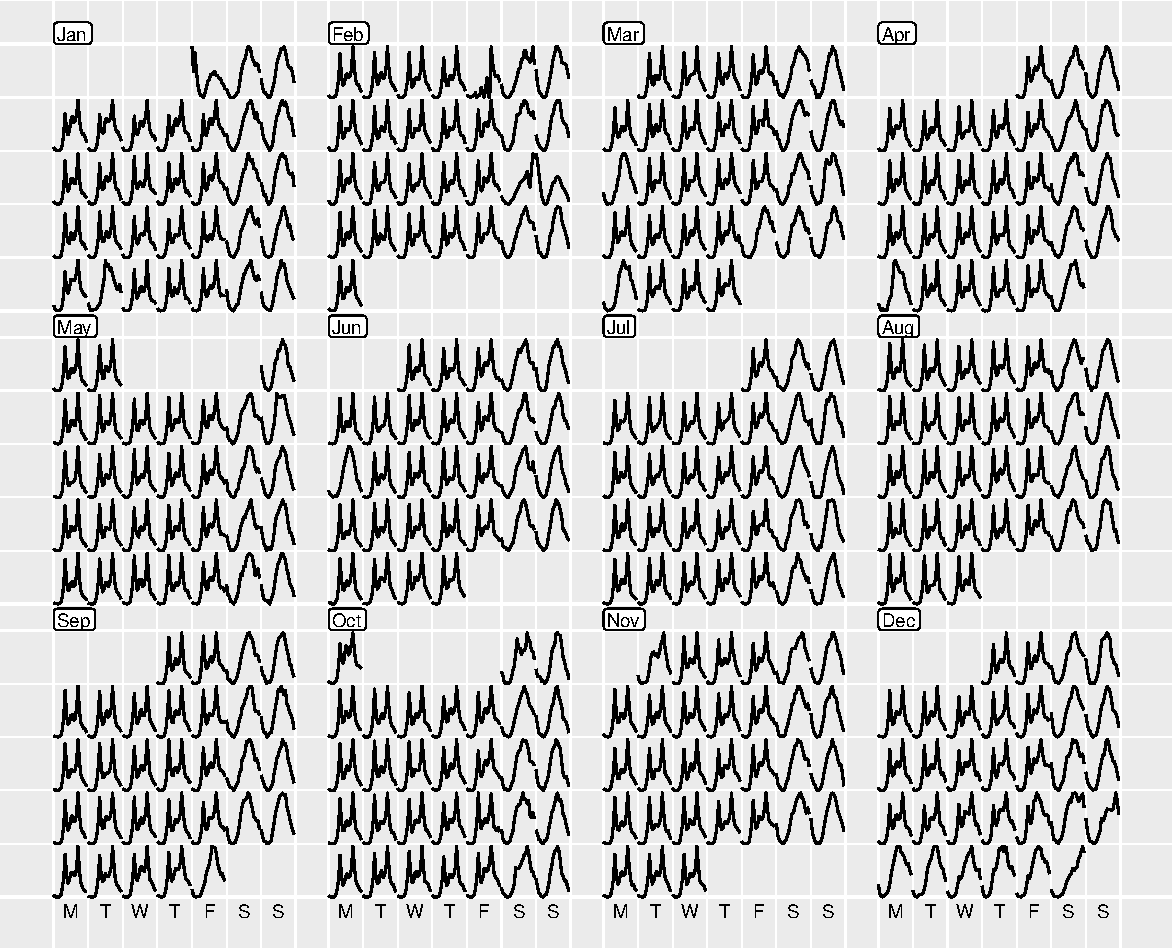
\includegraphics[width=\textwidth]{figure/flinders-free-1} 

}

\caption[Line glyphs on the calendar format showing hourly foot traffic at Flinders Street Station, scaled over all the days]{Line glyphs on the calendar format showing hourly foot traffic at Flinders Street Station, scaled over all the days. The individual shape on a single day becomes more distinctive, however it is impossible to compare the size of peaks between days.}\label{fig:flinders-free}
\end{figure}
\end{Schunk}

\hypertarget{orientation}{%
\subsection{Orientation}\label{orientation}}

By default, grids are laid out horizontally. This can be transposed by
setting the \code{dir} parameter to \code{"v"}, in which case \(i\) and
\(j\) are swapped in the Equation \ref{eq:grid}. This can be useful for
creating calendar layouts for countries where vertical layout is the
convention.

\hypertarget{language-support}{%
\subsection{Language support}\label{language-support}}

Most countries have adopted this western calendar layout, while the
languages used for week day and month would be different across
countries. We also offer languages other than English for text
labelling. Figure \ref{fig:chn-embedded} shows the same plot as Figure
\ref{fig:boxplot} labelled using simplified Chinese characters.

\hypertarget{variations}{%
\section{Variations}\label{variations}}

\label{sec:examples}

\hypertarget{overlaying-and-faceting-subsets}{%
\subsection{Overlaying and faceting
subsets}\label{overlaying-and-faceting-subsets}}

Plots can be layered. The comparison of sensors can be done by
overlaying plot the values for each (Figure \ref{fig:overlay}).
Differences between the pedestrian patterns for Flinders Street and
Flagstaff train stations can be seen. Both Flinders Street and Flagstaff
train stations exhibit strong commuters patterns, however, Flinders
Street has higher pedestrian counts during the weekends and public
holidays. This suggests that Flagstaff Station has limited functionality
on non-work days, but other activities occur around the Flinders Street
Station. From Figure \ref{fig:overlay} it can be seen that the State
Library has a similar temporal trend to Flinders Street Station on
non-work days. The nighttime events, such as White Night and New Year's
Eve, have barely affected the operation of Flagstaff Station but heavily
affected the incoming and outgoing traffic to Flinders Street Station
and the State Library.

\begin{Schunk}
\begin{figure}

{\centering 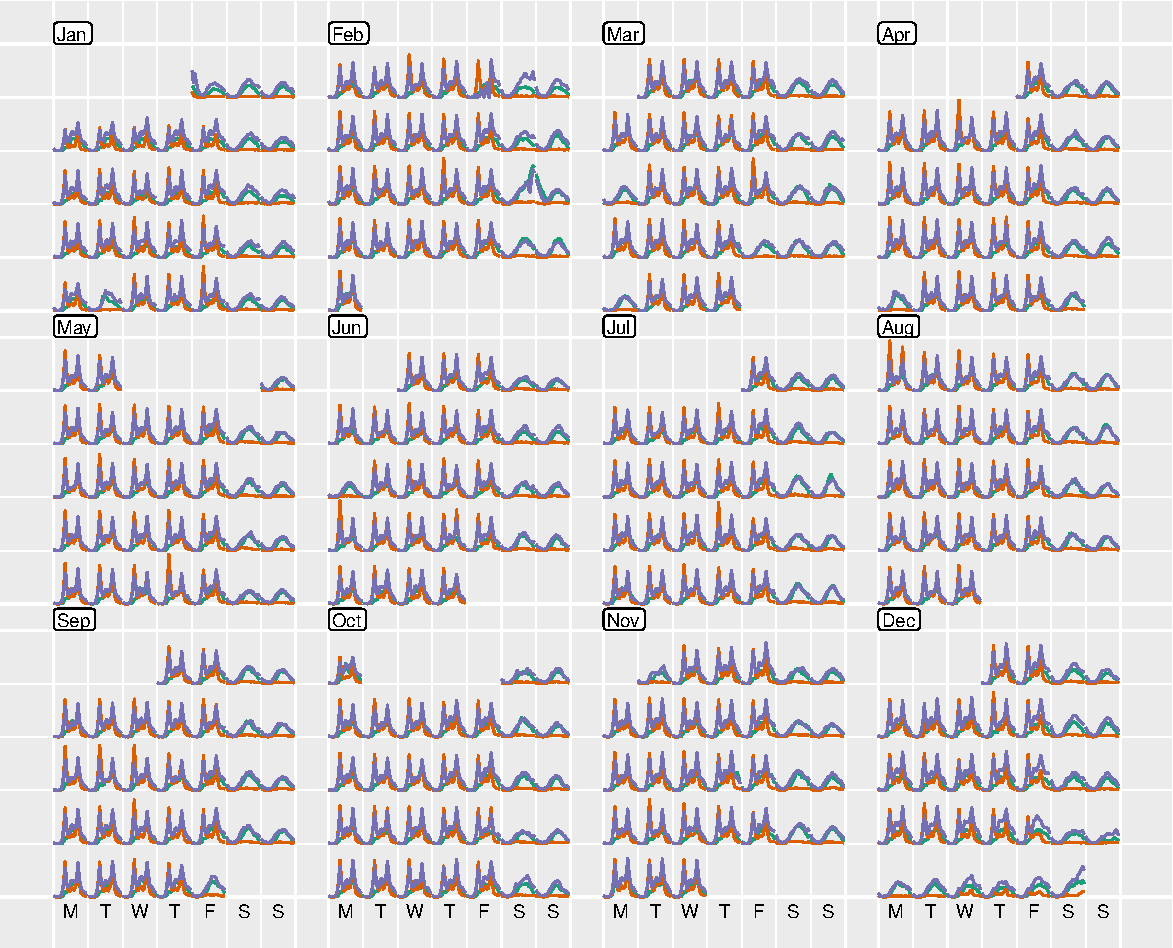
\includegraphics[width=\textwidth]{figure/overlay-1} 

}

\caption[Overlaying line graphs of the 3 sensors in the monthly calendar]{Overlaying line graphs of the 3 sensors in the monthly calendar. Flagstaff station is not as busy as the other two on non-work days.}\label{fig:overlay}
\end{figure}
\end{Schunk}

To avoid the overlapping problem, the calendar layout can be embedded
into a series of subplots for the different sensors. Figure
\ref{fig:facet} presents the idea of faceting calendar plots. This
allows comparing the overall structure between sensors, while
emphasising individual sensor variation.

\begin{Schunk}
\begin{figure}

{\centering 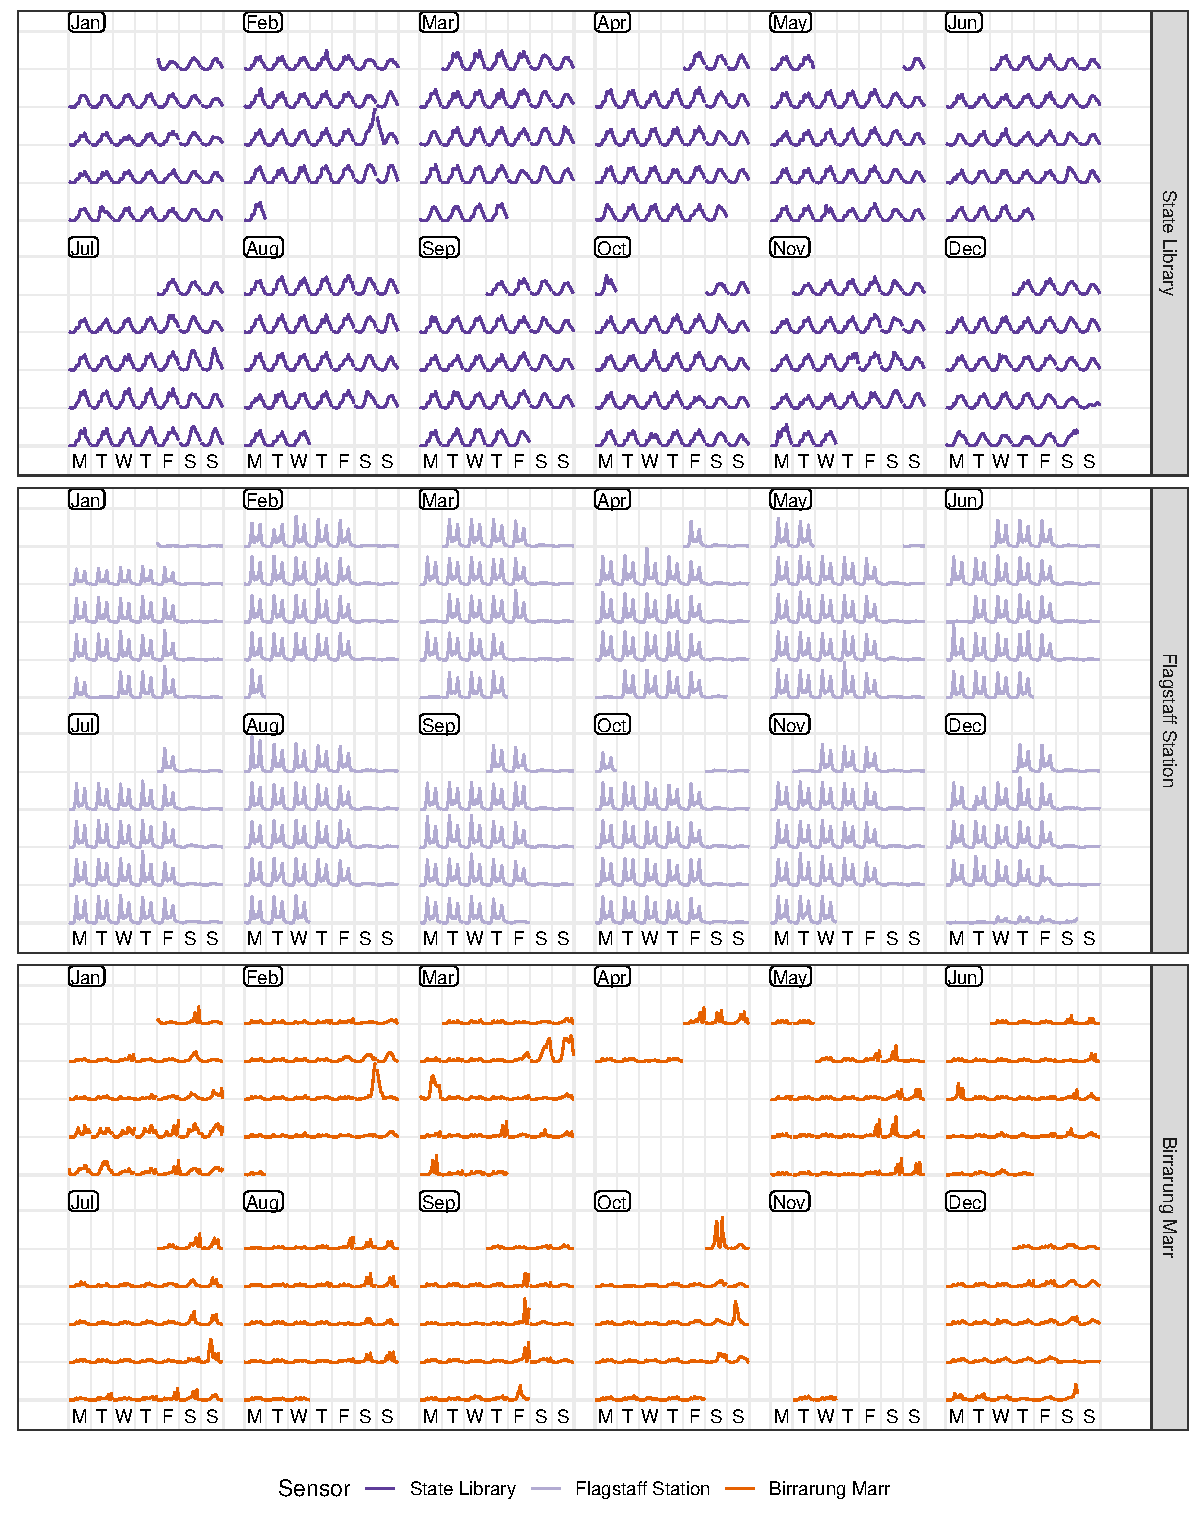
\includegraphics[width=\textwidth]{figure/facet-1} 

}

\caption[Line charts, embedded in the 6 by 2 monthly calendar, colored and faceted by the 3 sensors]{Line charts, embedded in the 6 by 2 monthly calendar, colored and faceted by the 3 sensors. The variations of an individual sensor are emphasised, and the shapes can be compared across the cells and sensors.}\label{fig:facet}
\end{figure}
\end{Schunk}

\hypertarget{different-types-of-plots}{%
\subsection{Different types of plots}\label{different-types-of-plots}}

The \code{frame\_calendar} function is not constrained to line plots.
The full range of plotting capabilities in \pkg{ggplot2} is essentially
available. Figure \ref{fig:scatterplot} shows a lag scatterplot at
Flinders Street Station, where the lagged hourly count is assigned to
the \code{x} argument and the current hourly count to the \code{y}
argument. This figure is organized in the daily calendar layout. Figure
\ref{fig:scatterplot} indicates two primary patterns, strong
autocorrelation on weekends, and weaker autocorrelation on work days. At
the higher counts, on week days, the next hour sees possibly substantial
increase or decrease in counts, essentially revealing a bimodal
distribution of consecutive counts, as supported by Figure
\ref{fig:flinders-2016}.

\begin{Schunk}
\begin{figure}

{\centering 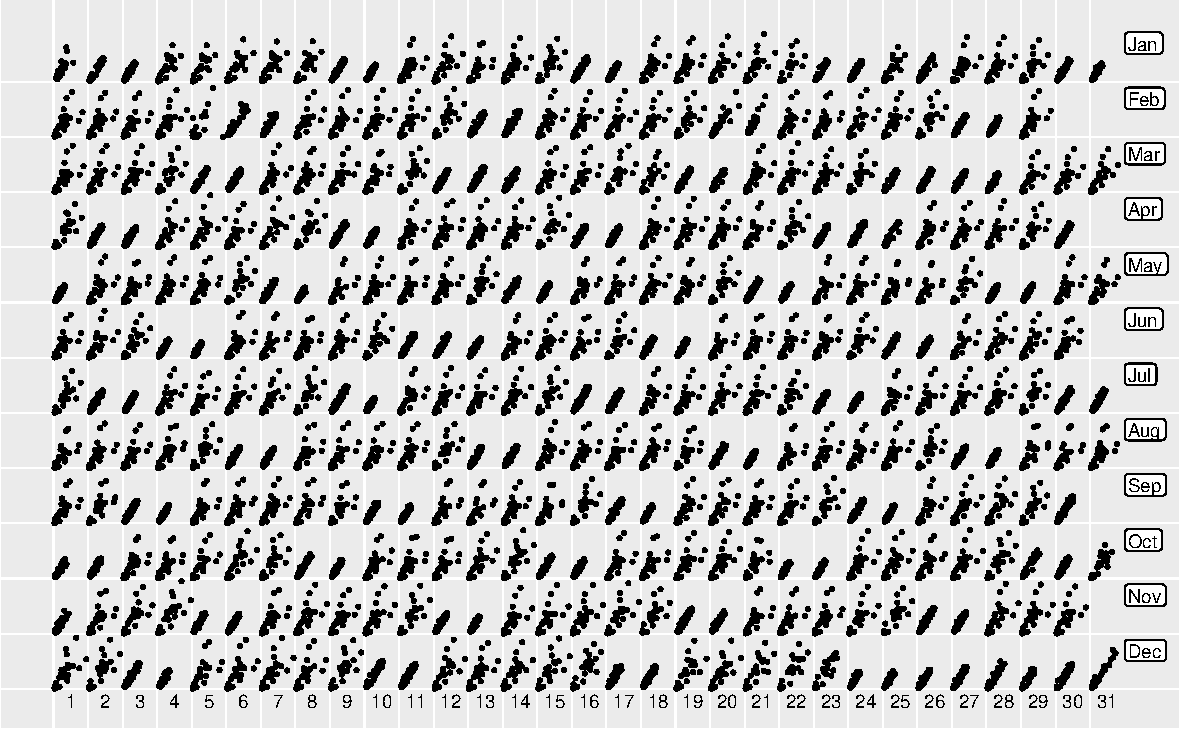
\includegraphics[width=\textwidth]{figure/scatterplot-1} 

}

\caption[Lag scatterplot in the daily calendar layout]{Lag scatterplot in the daily calendar layout. Each hour's count is plotted against previous hour's count at Flinders Street Station to demonstrate the autocorrelation at lag 1. The correlation between them is more consistent on non-work days than work days.}\label{fig:scatterplot}
\end{figure}
\end{Schunk}

The algorithm can also produce more complicated plots, such as boxplots.
Figure \ref{fig:boxplot} uses a loess smooth line superimposed on
side-by-side boxplots. It shows the distribution of hourly counts across
all 43 sensors during December. The last week of December is the holiday
season: people are off work on the day before Christmas, go shopping on
the Boxing day, and stay out for the fireworks on New Year's Eve.

\begin{Schunk}
\begin{figure}

{\centering 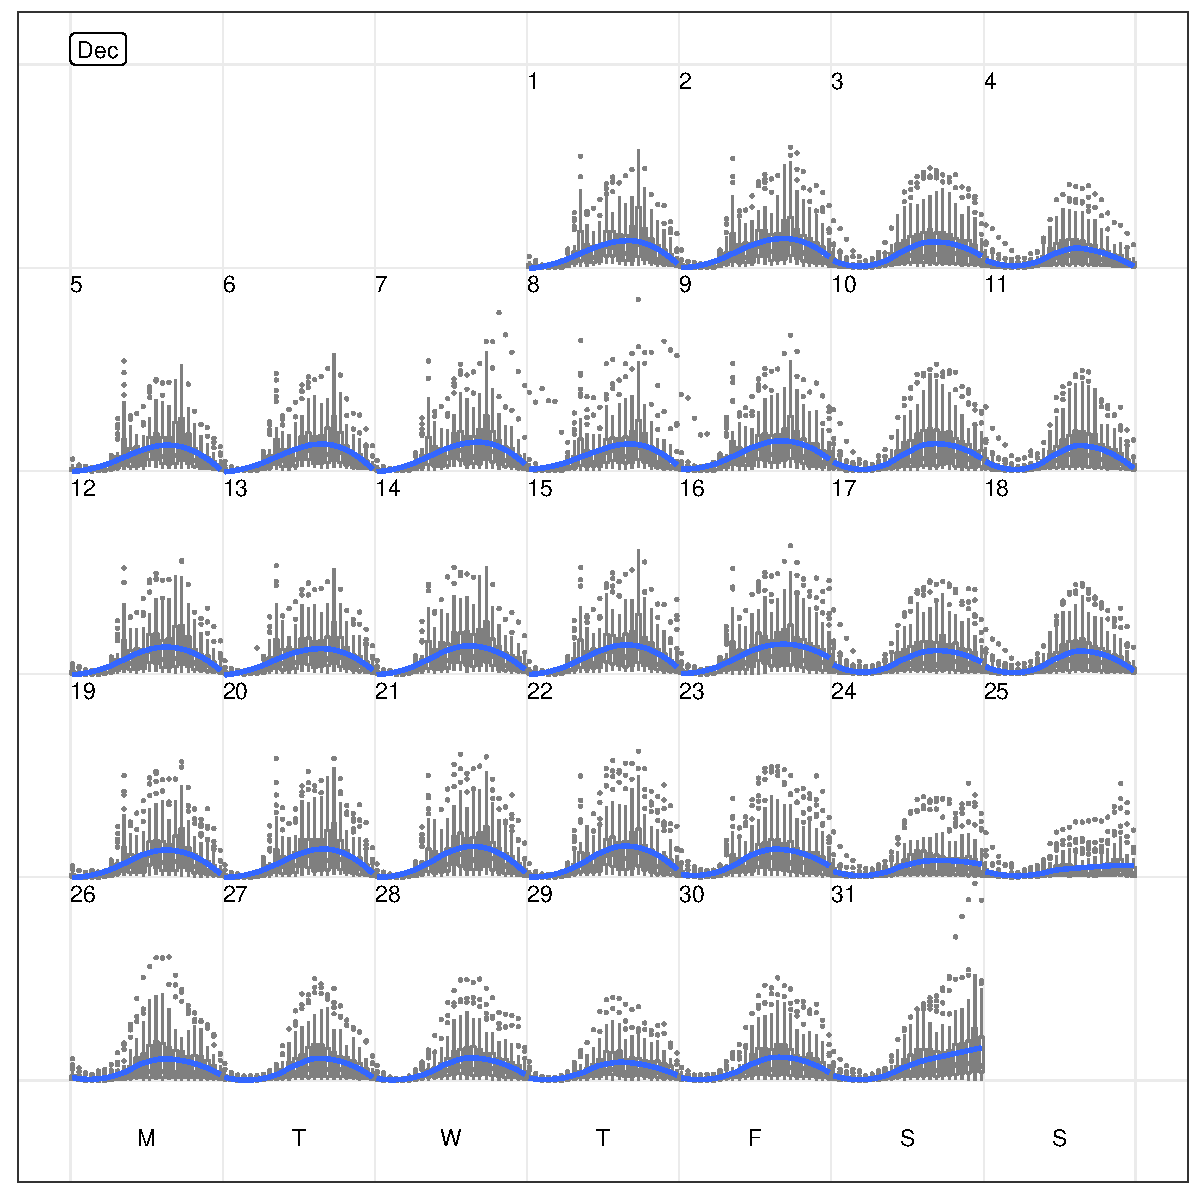
\includegraphics[width=\textwidth]{figure/boxplot-1} 

}

\caption[Side-by-side boxplots of hourly counts for all the 43 sensors in December 2016, with the loess smooth line superimposed on each day]{Side-by-side boxplots of hourly counts for all the 43 sensors in December 2016, with the loess smooth line superimposed on each day. It shows the hourly distribution in the city as a whole. There is one sensor attracting a larger number of people on New Year's Eve than the rest.}\label{fig:boxplot}
\end{figure}
\end{Schunk}

\begin{Schunk}
\begin{figure}

{\centering 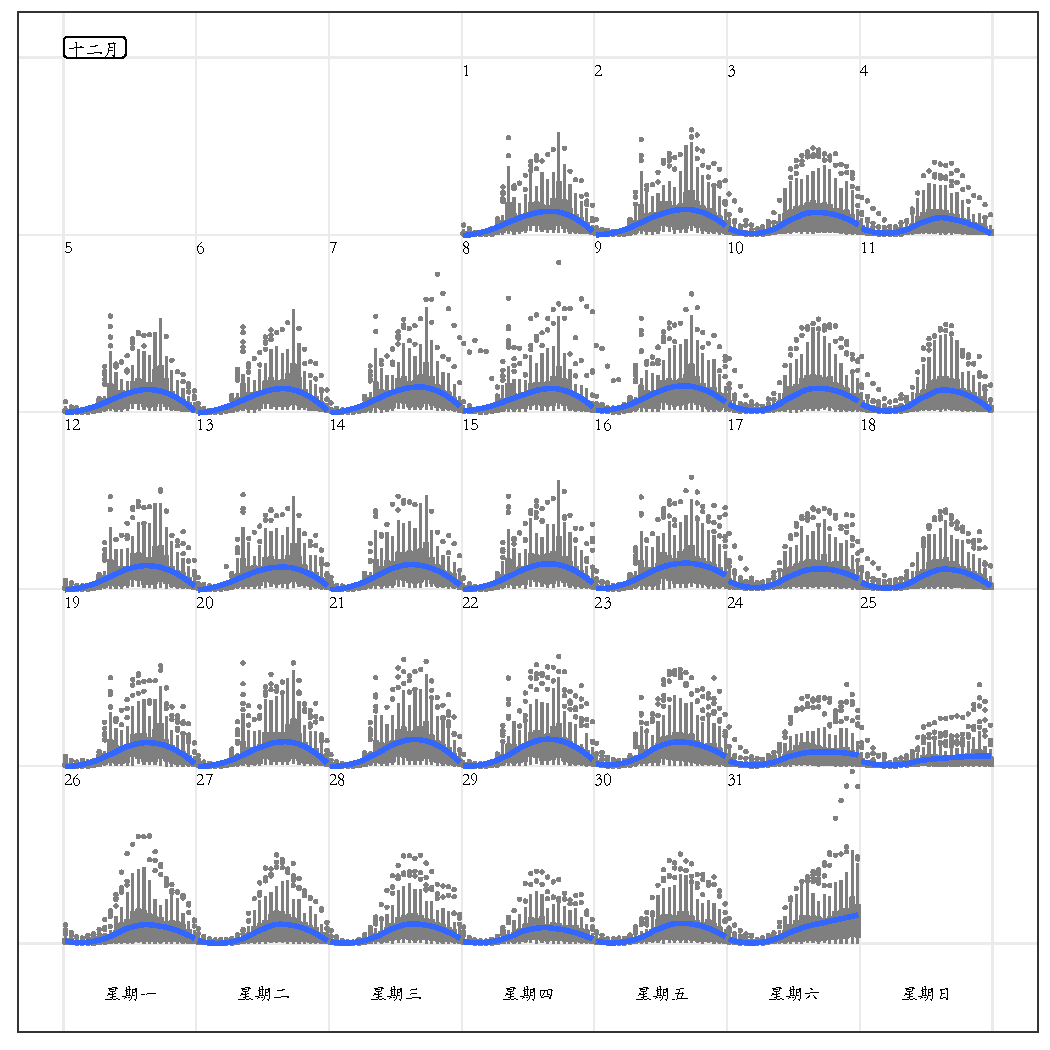
\includegraphics[width=\textwidth]{img/chn-1-embedded} 

}

\caption{The same plot as Figure \ref{fig:boxplot}, but with the month and week day labels in Chinese. It demonstrates the natural support for languages other than English.}\label{fig:chn-embedded}
\end{figure}
\end{Schunk}

\hypertarget{discussion}{%
\section{Discussion}\label{discussion}}

\label{sec:discussion}

The calendar-based visualization provides data plots in the familiar
format of an everyday tool. Patterns on special events for the region,
like Anzac Day in Australia, or Thanksgiving Day in the USA, more easily
pop out to the viewer as public holidays, than they would on a more
commonly used week day and month faceted layout.

The focus is on the western calendar layout, because most countries have
adopted this format. However the language of labels would differ across
countries, and so support was added for changing the label language
simply.

This sort of layout will be useful for studying consumer trends, or
human behavior, such as pedestrian patterns or pollution peaks. It will
not be so useful for physical patterns like temperature, which are not
typically affected by human activity. The layout does not replace
traditional displays, but serves to complement to further tease out
structure in temporal data. Analysts would still be advised to plot
overall summaries and deviations, in order to study general trends.

The layout is achieved by utilizing linear combinations of temporal
components and measured variables. This provides the data with the most
screen real estate. It could be useful to develop this into a
fully-fledged faceting method, with formal labels and axes. This is a
future goal.

\hypertarget{bibliography}{%
\section*{Bibliography}\label{bibliography}}
\addcontentsline{toc}{section}{Bibliography}

\hypertarget{refs}{}
\leavevmode\hypertarget{ref-ped}{}%
City of Melbourne. 2017. \emph{Pedestrian Volume in Melbourne}. City of
Melbourne, Australia. \url{http://www.pedestrian.melbourne.vic.gov.au}.

\leavevmode\hypertarget{ref-cleveland1984graphical}{}%
Cleveland, William S, and Robert McGill. 1984. ``Graphical Perception:
Theory, Experimentation, and Application to the Development of Graphical
Methods.'' \emph{Journal of the American Statistical Association} 79
(387). Taylor \& Francis: 531--54.

\leavevmode\hypertarget{ref-R-geofacet}{}%
Hafen, Ryan. 2018. \emph{Geofacet: 'Ggplot2' Faceting Utilities for
Geographical Data}. \url{https://CRAN.R-project.org/package=geofacet}.

\leavevmode\hypertarget{ref-R-ggcal}{}%
Jacobs, Jay. 2017. \emph{Ggcal: Calendar Plot Using Ggplot2}.
\url{https://github.com/jayjacobs/ggcal}.

\leavevmode\hypertarget{ref-R-ggTimeSeries}{}%
Kothari, Aditya, and Ather. 2016. \emph{ggTimeSeries: Nicer Time Series
Visualisations with Ggplot Syntax.}
\url{https://github.com/Ather-Energy/ggTimeSeries}.

\leavevmode\hypertarget{ref-lam2007overview}{}%
Lam, Heidi, Tamara Munzner, and Robert Kincaid. 2007. ``Overview Use in
Multiple Visual Information Resolution Interfaces.'' \emph{IEEE
Transactions on Visualization and Computer Graphics} 13 (6). IEEE:
1278--85.

\leavevmode\hypertarget{ref-VanWijkCluster1999}{}%
Van Wijk, Jarke J., and Edward R. Van Selow. 1999. ``Cluster and
Calendar Based Visualization of Time Series Data.'' In \emph{Information
Visualization, 1999. INFOVIS 1999 Proceedings. IEEE Symposium on}, 4--9.
IEEE.

\leavevmode\hypertarget{ref-R-sugrrants}{}%
Wang, Earo, Di Cook, and Rob Hyndman. 2018. \emph{Sugrrants: Supporting
Graphs for Analysing Time Series}. \url{https://pkg.earo.me/sugrrants}.

\leavevmode\hypertarget{ref-wickham2009ggplot2}{}%
Wickham, Hadley. 2009. \emph{Ggplot2: Elegant Graphics for Data
Analysis}. New York, NY: Springer-Verlag New York.

\leavevmode\hypertarget{ref-wickham2014tidy}{}%
---------. 2014. ``Tidy Data.'' \emph{Journal of Statistical Software}
59 (10). Foundation for Open Access Statistics: 1--23.

\leavevmode\hypertarget{ref-R-tidyverse}{}%
---------. 2017. \emph{Tidyverse: Easily Install and Load the
'Tidyverse'}. \url{https://CRAN.R-project.org/package=tidyverse}.

\leavevmode\hypertarget{ref-R-ggplot2}{}%
Wickham, Hadley, Winston Chang, Lionel Henry, Thomas Lin Pedersen,
Kohske Takahashi, Claus Wilke, and Kara Woo. 2018. \emph{Ggplot2: Create
Elegant Data Visualisations Using the Grammar of Graphics}.

\leavevmode\hypertarget{ref-Wickham2012glyph}{}%
Wickham, Hadley, Heike Hofmann, Charlotte Wickham, and Dianne Cook.
2012. ``Glyph-Maps for Visually Exploring Temporal Patterns in Climate
Data and Models.'' \emph{Environmetrics} 23 (5): 382--93.

\leavevmode\hypertarget{ref-wilkinson2006grammar}{}%
Wilkinson, Leland. 2005. \emph{The Grammar of Graphics (Statistics and
Computing)}. Secaucus, NJ: Springer-Verlag New York, Inc.

\bibliography{RJreferences.bib}

\address{%
Earo Wang\\
Monash University\\
Department of Econometrics and Business Statistics,\\ Monash University, VIC 3800\\ Australia\\
}
\href{mailto:earo.wang@monash.edu}{\nolinkurl{earo.wang@monash.edu}}

\address{%
Dianne Cook\\
Monash University\\
Department of Econometrics and Business Statistics,\\ Monash University, VIC 3800\\ Australia\\
}
\href{mailto:dicook@monash.edu}{\nolinkurl{dicook@monash.edu}}

\address{%
Rob J Hyndman\\
Monash University\\
Department of Econometrics and Business Statistics,\\ Monash University, VIC 3800\\ Australia\\
}
\href{mailto:rob.hyndman@monash.edu}{\nolinkurl{rob.hyndman@monash.edu}}

